\documentclass[margin=0px]{article}

\usepackage{listings}
\usepackage[utf8]{inputenc}
\usepackage{graphicx}
\usepackage{float}
\usepackage[a4paper, margin=0.7in]{geometry}
\usepackage{subcaption}
\usepackage{amsthm}
\usepackage{amssymb}
\usepackage{amsmath}
\usepackage{fancyhdr}
\usepackage{setspace}

\onehalfspacing

\renewcommand{\figurename}{ábra}
\newenvironment{tetel}[1]{\paragraph{#1 \\}}{}

\newcommand{\N}{\mathbb{N}}
\newcommand{\Z}{\mathbb{Z}}
\newcommand{\R}{\mathbb{R}}
\newcommand{\Q}{\mathbb{Q}}
\newcommand{\C}{\mathbb{C}}

\pagestyle{fancy}
\lhead{\it{PTI BSc Záróvizsga tételek}}
\rhead{4.1 Kódoláselmélet}

\title{\textbf{{\Large ELTE IK - Programtervező Informatikus BSc} \vspace{0.2cm} \\ {\huge Záróvizsga tételek}} \vspace{0.3cm} \\ 4.1 Kódoláselmélet}
\author{}
\date{}

\begin{document}
\maketitle

\section{Kódoláselmélet}
\subsection{Betűnkénti kódolás}
A kódolás a legáltalánosabb értelemben az üzentek halmazának egy másik halmazba való leképzését jelenti. Gyakran az üzenetet valamilyen karakterkészlet elemeiből alkotott sorozattal adjuk meg. Ekkor az üzenetet felbontjuk előre rögzített olyan elemi részekre, hogy minden üzenet egyértelműen előálljon ilyen elemi részek sorozataként. A kódoláshoz megadjuk az elemi részek kódját, amelyet egy szótár tartalmaz. Az ilyen kódolást betűnkénti kódolásnak nevezzük.

A kódolandó üzenetek egy $A$ ábécé betűi, és egy-egy betű kódja egy másik, $B$ ábécé (kódábécé) betűinek felel meg. Tegyük fel, hogy mind két ábécé nem üres és véges.

Egy $A$ ábécé betűiből felírható szavak halmazát $A^+$-szal jelöljük, míg az üres szóval kiterjesztettet $A^*$-gal.

Ez alapján a betűnkénti kódolást egy $\varphi: A \rightarrow B^*$ leképezés határozza meg, amelyet kiterjeszthetünk egy $\psi: A^* \rightarrow B^*$ leképezéssé, alábbi módon: Ha $\alpha_1\alpha_2...\alpha_n = \alpha \in A$, akkor $\alpha$ kódja $\psi(\alpha) = \varphi(\alpha_1)\varphi(\alpha_2)...\varphi(\alpha_3)$. Nyilván ha $\varphi$ nem injektív (vagy az üres szó benne van az értékkészletében), akkor a $\psi$ kódolás sem injektív, azaz nem egyértelműen dekódolható. Emiatt feltehetjük, hogy $\varphi$ injektív, és $B^+$-ba képez.

\subsection{Shannon- és Huffman-kód}
\begin{description}
    \item[Alapfogalmak] \hfill
        \begin{itemize}
            \item Gyakoriság, relatív gyakoriság, eloszlás \\
                  Az információforrás $n$ üzenetet bocsájt ki. A különböző üzeneteket jelöljük $a_1, \cdots, a_m$-mel. $a_i$ üzenet $k_i$-szer fordul elő, melyet gyakoriságnak nevezzük. Az $a_i$ relatív gyakorisága a $p_i = k_i/n$. A $p_1,\cdots,p_m$ szám $m$-est az üzentek eloszlásának nevezzük. ($\sum_{i=1}^{m}p_i = 1$)
            \item Információtartalom \\
                  Az $a_i$ üzenet egyedi információtartalma $I_i = - \text{log}_rp_i$, ahol $r>1$ az információ egysége. ($r=2$ esetén az egység a bit).
            \item Entrópia \\
                  Az üzenetforrás által kibocsátott átlagos információtartalmat nevezzük entrópiának:
                  \[H_r(p_1, \cdots, p_m) = - \sum\limits_{i=1}^{m}p_i\text{log}_rp_i  \]
            \item Prefix, szuffix, infix \\
                  Legyen $\alpha, \beta, \gamma \in A$ szavak. Ekkor az $\alpha\beta\gamma$ szónak $\alpha$ prefixe, $\beta$ infixe, $\gamma$ pedig szuffixe.
            \item Kódfa \\
                  A betűnkénti kódoláshoz egyértelműen adható meg egy szemléletes irányított, élcímkézett fa. Legyen $\varphi : A \rightarrow B^*$ a betűnkénti kódolás. Készítsünk el egy olyan fát, melynek a gyökere az üres szó és ha $\beta = \alpha b\quad (b\in B)$-re, akkor $\alpha$-ból húzódjon olyan él $\beta$-ba, melynek $b$ címkéje van. Ekkor minden azonos hosszú szó egy szinten lesz. Azokat a csúcsokat, melyekből minden $b\in B$ címkével vezet ki él teljes csúcsnak nevezzük, különben csonka csúcsok.
            \item Prefix kód, egyenletes kód, vesszős kód \\
                  A $\varphi : A \rightarrow B^+$ injektív leképezés által meghatározott $\psi : A^* \rightarrow B^*$ betűnkénti kódolás
                  \begin{enumerate}
                      \item felbontható (egyértelműen dekódolható), ha $\psi$ injektív
                      \item prefix kód, ha $\varphi$ értékkészlete prefixmentes.
                      \item egyenletes kód (fix hosszúságú), ha $\psi$ értékkészletében minden elem megegyező hosszú
                      \item vesszős kód, ha $\exists \vartheta \in B^+$ vessző, hogy $\vartheta$ szuffixe minden kódszónak, de sem prefixe, sem infixe semelyik kódszónak.
                  \end{enumerate}
            \item Átlagos szóhosszúság \\
                  Legyen $A = \{a_1,\cdots, a_n\}$ a kódolandó ábécé. Az $a_i$ kódjának hossza $l_i$. Ekkor $\overline{l} = \sum_{i=1}^{n}p_il_i$ a kód átlagos szóhosszúsága.
            \item Optimális kód \\
                  Ha egy adott elemszámú ábécével és adott eloszlással egy felbontható betűnkénti kód átlagos szóhoszúsága minimális, akkor optimális kódnak nevezzük.
        \end{itemize}
    \item[Shannon-kód] \hfill \\
        Shannon kód egy optimális kód ($r$ elemszámú ábécével és $p_i$ gyakoriságokkal), melyet a következő módon állítunk elő.
        \begin{enumerate}
            \item Rendezzük a betűket relatív gyakoriságaik alapján csökkenő sorrendbe.
            \item Határozzuk meg az $l_1,\cdots,l_n$ szóhosszúságokat a következő módon:
                  \[r^{-l_i} \leq p_i < r^{-l_i+1} \]
            \item Osszuk el az ábécé elemeit az egyes helyiértékeken.
        \end{enumerate}
        Példa:

        Legyen a kódábécé a ${0,1,2}$ halmaz, az kódolandó betűk és gyakoriságaik pedig a következők:

        \begin{tabular}{|c|c|c|c|c|c|c|c|c|c|}
            \hline a    & b    & c    & d    & e    & f    & g    & h    & i    & j    \\
            \hline 0,17 & 0,02 & 0,13 & 0,02 & 0,01 & 0,31 & 0,02 & 0,17 & 0,06 & 0,09 \\
            \hline
        \end{tabular}

        A relatív gyakoriságok rendezése után:

        \begin{tabular}{|c|c|c|c|c|c|c|c|c|c|}
            \hline f    & a    & h    & c    & j    & i    & b    & d    & g    & e    \\
            \hline 0,31 & 0,17 & 0,17 & 0,13 & 0,09 & 0,06 & 0,02 & 0,02 & 0,02 & 0,01 \\
            \hline
        \end{tabular}

        Határozzuk meg szóhosszúságokat. Az f, a, h és c esetében: $3^{-2} = r^{-l_i} \leq p_i < r^{-l_i+1} = 3^{-1} $ Tehát azok szóhosszúsága 2. A többi esetben is így járunk el:

        \begin{tabular}{|c|c|c|c|c|c|c|c|c|c|}
            \hline f    & a    & h    & c    & j    & i    & b    & d    & g    & e    \\
            \hline 0,31 & 0,17 & 0,17 & 0,13 & 0,09 & 0,06 & 0,02 & 0,02 & 0,02 & 0,01 \\
            \hline 2    & 2    & 2    & 2    & 3    & 3    & 4    & 4    & 4    & 5    \\
            \hline
        \end{tabular}

        Ezek alapján f kódszava a 00, a kódszava a 01, h-hoz a 02 tartozik, míg c-hez 10. A j-hez ezek után 11 tartozna, de mivel az 3 hosszú, így 110.
        A kódszavak tehát a következőképp alakulnak:

        \begin{tabular}{|c|c|c|c|c|c|c|c|c|c|}
            \hline f    & a    & h    & c    & j    & i    & b    & d    & g    & e     \\
            \hline 0,31 & 0,17 & 0,17 & 0,13 & 0,09 & 0,06 & 0,02 & 0,02 & 0,02 & 0,01  \\
            \hline 2    & 2    & 2    & 2    & 3    & 3    & 4    & 4    & 4    & 5     \\
            \hline 00   & 01   & 02   & 10   & 110  & 111  & 1120 & 1121 & 1122 & 12000 \\
            \hline
        \end{tabular}

        A kódfát \ref{fig:shannon}. ábrán láthatjuk.

        \begin{figure}[H]
            \centering
            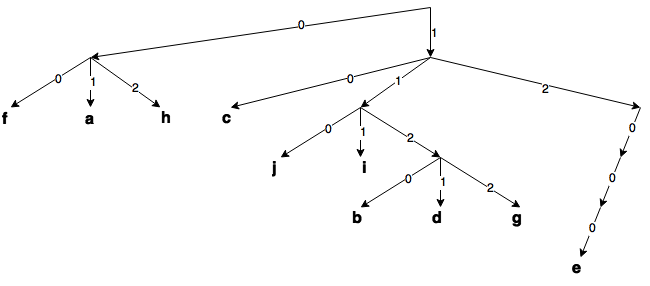
\includegraphics[width=0.6\textwidth]{img/shannon.png}
            \caption{Shannon-kód példa kódfája}
            \label{fig:shannon}
        \end{figure}

    \item[Huffman-kód] \hfill \\
        A Huffman-kód is optimális kód ($r$ elemszámú ábécével és $p_i$ gyakoriságokkal), melyet a következő módon állítunk elő.
        \begin{enumerate}
            \item Rendezzük a betűket relatív gyakoriságaik alapján csökkenő sorrendbe.
            \item Annak érdekében, hogy csak egy csonka csúcs keletkezzen
                  \[m \equiv n \mod{r-1}\]
                  kongruenciának teljesülnie kell, ahol $m$ az egyetlen csonka csúcs kifoka. Ami ekvivalens azzal, hogy $m = 2 + ((n-2) \mod{r-1})$. Tehát osszuk el $n-2$-t $r-1$-gyel, és így $m$ a maradék+2 lesz.
            \item Az első lépésben a sorozat $m$ utolsó betűjét összevonjuk (új jelölést/betűt adunk neki), és ennek a relatív gyakorisága a tagok relatív gyakoriságának összege lesz. Rendezzük a sorozatot. Ezen lépés után már a betűk száma kongruens $r-1$-gyel, így a következő redukciós lépésekben mindig teljes csúcsokat tudunk készíteni.
            \item \label{itm:huffman_red} Az utolsó $r$ betűt vonjunk össze, helyettesítsük egy új betűvel és relatív gyakoriság legyen a relatív gyakoriságok összege.
            \item A \ref{itm:huffman_red}-beli redukciós lépést addig ismételjük míg $r$ db betű nem marad. Ekkor rendre minden betűhöz a kódábécé egy-egy betűjét rendeljük.
            \item \label{itm:huffman_split} Ha redukált elemmel találkozunk szétbontjuk, majd az ő elemeihez is a kódábécé betűit rendeljük, de konkatenáljuk az előzővel.
            \item A \ref{itm:huffman_split}-beli lépést addig ismételjük míg marad redukált elem.
        \end{enumerate}

        Példa:

        A Shannon-kódnál látott forrást kódoljuk be ugyanúgy $\{0,1,2\}$ kódábécével.

        \begin{tabular}{|c|c|c|c|c|c|c|c|c|c|}
            \hline a    & b    & c    & d    & e    & f    & g    & h    & i    & j    \\
            \hline 0,17 & 0,02 & 0,13 & 0,02 & 0,01 & 0,31 & 0,02 & 0,17 & 0,06 & 0,09 \\
            \hline
        \end{tabular}

        Rendezzük relatív gyakoriság szerint:

        \begin{tabular}{|c|c|c|c|c|c|c|c|c|c|}
            \hline f    & a    & h    & c    & j    & i    & b    & d    & g    & e    \\
            \hline 0,31 & 0,17 & 0,17 & 0,13 & 0,09 & 0,06 & 0,02 & 0,02 & 0,02 & 0,01 \\
            \hline
        \end{tabular}

        Osszuk el $n-2$-t $r-1$-gyel: $10-2 = 4*(3-1)+0$. Így $m$ a maradék+2, azaz $m=2$.
        Az utolsó $m$ betűt összevonjuk, és rendezzük a sorozatot:

        \begin{tabular}{|c|c|c|c|c|c|c|c|c|}
            \hline f    & a    & h    & c    & j    & i    & (g,e) & b    & d    \\
            \hline 0,31 & 0,17 & 0,17 & 0,13 & 0,09 & 0,06 & 0,03  & 0,02 & 0,02 \\
            \hline
        \end{tabular}

        Innentől kezdve minden redukciós lépésben az utolsó $r$ db azaz 3 betűt vonjuk össze:

        \begin{tabular}{|c|c|c|c|c|c|c|}
            \hline f    & a    & h    & c    & j    & ((g,e), b, d) & i    \\
            \hline 0,31 & 0,17 & 0,17 & 0,13 & 0,09 & 0,07          & 0,06 \\
            \hline
        \end{tabular}

        Ezt addig ismételjük, míg $r$ darab betű marad:

        \begin{tabular}{|c|c|c|}
            \hline (a,h,c) & f    & (j,((g,e),b,d),i) \\
            \hline 0,47    & 0,31 & 0,22              \\
            \hline
        \end{tabular}

        A szétbontás alapján a \ref{fig:huffmann_split}. ábrán látható fát tudjuk összeállítani.

        \begin{figure}[H]
            \centering
            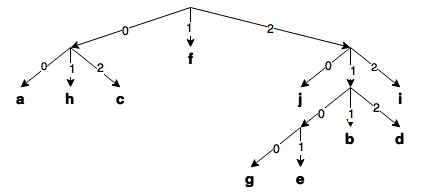
\includegraphics[width=0.6\textwidth]{img/huffmann_split.png}
            \caption{Huffman-kód példa kódfája}
            \label{fig:huffmann_split}
        \end{figure}

        Ezek alapján a kódtábla:

        \begin{tabular}{|c|c|c|}
            \hline betű & gyakoriság & kód  \\
            \hline f    & 0,31       & 1    \\
            \hline a    & 0,17       & 00   \\
            \hline h    & 0,17       & 01   \\
            \hline c    & 0,13       & 02   \\
            \hline j    & 0,09       & 20   \\
            \hline i    & 0,06       & 22   \\
            \hline b    & 0,02       & 211  \\
            \hline d    & 0,02       & 212  \\
            \hline g    & 0,02       & 2100 \\
            \hline e    & 0,01       & 2101 \\
            \hline
        \end{tabular}
\end{description}
\subsection{Hibajavító kódok, kódtávolság}
\begin{description}
    \item[Hibakorlátozó kódolás] \hfill \\
        A hibakorlátozó kódokat két csoportba sorolhatjuk: hibajelző és  hibajavító kódok. Mindkét esetben az üzenetekhez kódszavakat rendelünk, amik alapján az átvitel során keletkező hibákat kezelni tudjuk. Ha az üzenet könnyen ismételhető hibajelző, ha nehezen ismételhető hibajavító kódot alkalmazunk. A hibakorlátozó kódoknál mindig azonos hosszúságú kódszavakat használunk.
    \item[Kódok távolsága, súlya] \hfill \\
        A kódábécé $u$ és $v$ szavának Hamming-távolsága $d(u,v)$ az azonos pozícióban levő, eltérő jegyek száma.  A Hamming-távolság rendelkezik a távolság szokásos tulajdonságaival, vagyis $\forall u,v,z$:
        \begin{itemize}
            \item $d(u,v) \geq 0$
            \item $d(u,v) = 0 \ \Longleftrightarrow \ u = v$
            \item $d(u,v) = d(v,u)$ - szimmetria
            \item $d(u,z) \leq d(u,v)+d(v,z)$ - háromszög egyenlőtlenség
        \end{itemize}
        A kód távolsága $d(C) = \min\limits_{u\neq v}d(u,v) \qquad (u,v \in C)$

        Amennyiben az $A$ kódábécé Abel-csoport a $0$ nullelemmel. Ekkor egy $u$ szó Hamming-súlya ($w(u)$) a szóban szereplő nem nulla elemek száma. Ekkor a kód súlya $w(C)  = \min\limits_{u\neq 0}w(u)$
    \item[Hibajavító kód] \hfill \\
        Amikor egy olyan szót kapunk, ami nem kódszó, a hozzá legkisebb Hamming-távolságú kódszóra javítjuk.

        A $K$ kód $t$-hibajavító, ha egy legfeljebb $t$ helyen megváltozott kódot helyesen javít. A $K$ kód pontosan $t$-hibajavító, ha $t$-hibajavító, de nem $t+1$-hibajavító.

        \textit{Megjegyzés: d minimális távolságú kód esetén d/2-nél kevesebb hibát biztosan egyértelműen tudunk javítani.}
    \item[Hamming-korlát] \hfill \\
        Egy $q$ elemű ábécé $n$ hosszú szavaiból álló $C$ kód $t$-hibajavító. Ekkor bármely két kódszóra a tőlünk legfeljebb $t$ távolságra lévő szavak halmazai diszjunktak.

        Mivel egy kódszótól $j$ távolságra pontosan $\binom{n}{j}(q-1)^j$ szó van, így a Hamming-korlát a kódszavak számára adott $t$-nél:
        \[\#(C) \cdot \sum\limits_{j=0}^{t}\binom{n}{j}(q-1)^j \leq q^n \]

        Amennyiben egyenlőség áll fent tökéletes kódról beszélünk.
\end{description}
\subsection{Lineáris kódok}
\begin{description}
    \item[Definíció] \hfill \\
        $A$ véges test és $A^n$ lineáris tér. Minden $ K \leq A^n$ alteret lineáris kódnak nevezzük. Ha az altér $k$ dimenziós, a kód távolsága $d$ és $\#(A) = q$, akkor az ilyen kódot $[n,k,d]_q$ kódnak nevezzük.

        Egy lineáris kódnál feltesszük, hogy kódolandó üzenetek $K^k$ elemei, azaz a kódábécé elemeiből képzett $k$-asok.
    \item[Generátormátrix] \hfill \\
        $K$ véges test feletti $[n,k,d]_q$ lineáris kódolást válasszuk egy (kölcsönösen egyértelmű) lineáris leképezésnek:
        \[ G:K^k \rightarrow K^n \]
        Ezt egy mátrixszal, az úgy nevezett generátormátrixszal jellemezhetjük.
    \item[Polinomkódok] \hfill \\
        Egy lineáris kód esetén az üzeneteket megfeleltethetjük $\mathbb{F}_q$ ($q$ elemű véges test) feletti $k$-nál alacsonyabb fokú polinomoknak.
        \[(a_0,a_1,\cdots,a_{k-1}) \rightarrow a_0+a_1x+\cdots+a_{k-1}x^{k-1} \]

        Legyen $g(x)$ rögzített $m$-edfokú polinom. A $p(x)$ polinomot (üzenet) $g(x)$-szel szorozva lineáris kódolást kapunk (mivel a $p \rightarrow pg$ kölcsönösen egyértelmű). Ekkor a kódszavak hossza $n=k+m$. Az ilyen típusú lineáris kódolást polinomkódolásnak nevezzük.

        \textit{Megjegyzés: Feltehetjük, hogy $g(x)$ főpolinom (együtthatója egység), illetve a konstans tag nem nulla (ha nulla lenne, a szorzatban kiesne a konstans tag, így a kódban a nulla indexű betű soha nem hordozna információt)}
    \item[CRC - Cyclic Redundancy Check] \hfill \\
        Ha egy polinomkódban $g(x) | x^n-1$, akkor ciklikus kódról beszélünk. Ekkor, ha $a_0a_1\cdots a_{n-1}$ kódszó, akkor $a_{n-1}a_0\cdots a_{n-2}$ is az, mivel:
        \[ a_{n-1}+a_0x+\cdots+a_{n-2}x^{n-1} \ = \ x\cdot(a_0+a_1x+\cdots a_{n-1}x^{n-1})-a_{n-1}(x^n-1) \]
        osztható $g(x)$-szel.

        A CRC az $\mathbb{F}_2$ feletti ciklikus kódokat foglalja magába. Csak hibajelzésre alkalmas, a kódolás a következő: Vegyük $p(x)x^m = (0,0,\cdots,0,a_m,a_{m+1},\cdots,a_{n-1})$. Ezt osszuk el $g(x)$-el maradékosan. $p(x)x^m = q(x)g(x)+r(x)$. Ekkor a kódszó legyen: $p(x)x^m-r(x) = q(x)g(x)$, amely osztható $g(x)$-szel és magas fokszámokon az eredeti üzenet betűi helyezkednek el. A vett szó ellenőrzése egyszerű: Megnézzük, hogy osztható-e $g(x)$-szel, ha nem, hiba történt.
\end{description}

\end{document}